\documentclass[10pt,conference,compsocconf]{IEEEtran}
\usepackage{amssymb}
\usepackage{amsmath}
\usepackage{times}
\usepackage{caption}
\captionsetup{font=footnotesize,justification=centering,labelsep=period}
\usepackage{cite}
\usepackage[pdftex]{graphicx}
\usepackage{array}
\usepackage[english]{babel}
\usepackage[autostyle]{csquotes}
\usepackage[T1]{fontenc}
\MakeOuterQuote{"}
\parskip 3pt plus 2pt minus 1pt
\pagestyle{empty}
\begin{document}
\pagenumbering{gobble}

\title{\textbf{\Large An academic title}\\[0.2ex]}

\author{
\IEEEauthorblockN{~\\[-0.4ex]\large James Kirk, Captain\\[0.3ex]\normalsize}
\IEEEauthorblockA{Starfleet Academy\\San Francisco, California 5555}
\and
\IEEEauthorblockN{~\\[-0.4ex]\large Jean-Luc Picard, 1st Officer\\[0.3ex]\normalsize}
\IEEEauthorblockA{}}
\maketitle

\begin{abstract}
This article describes how to use the IEEEtran class with LaTeX to produce high
quality typeset papers that are suitable for submission to the Institute of
Electrical and Electronics Engineers (IEEE). IEEEtran can produce conference,
journal and technical note (correspondence) papers with a suitable choice of
class options. This document was produced using IEEEtran in journal mode.
\end{abstract}

\begin{IEEEkeywords}
Class, IEEEtran, LATEX, paper, style, template, typesetting.
\end{IEEEkeywords}

\section{Introduction}
\label{introduction}

\captionsetup{font={footnotesize,sc},justification=centering,labelsep=period}
\begin{table}[htbp]
\caption{List of Historical Figures}
\label{historicalFigures}
\centering
\begin{tabular}{lll}
\hline
\textit{foobar} & \textit{set amet} \\
\hline
f1 & \texttt{s1 || s2}\\
f2 & \texttt{s2 \&\& f2}\\
\hline
\end{tabular}
\end{table}
\captionsetup{font={footnotesize,rm},justification=centering,labelsep=period}

With a recent IEEEtran class file, a computer running LATEX, and a basic
understanding of the LATEX language, an author can produce professional quality
typeset research papers very quickly, inexpensively, and with minimal effort.
The purpose of this article is to serve as a user guide of Table~\ref{historicalFigures}
IEEEtran LATEX class and to document its unique features and behavior.

\begin{enumerate}
\item List item
\item Art
\item Echo fox tango
\end{enumerate}

This document applies to version 1.7 and later of IEEEtran. Prior versions do
not have all of the features described here. IEEEtran will display the version
number on the user’s console when a document using it is being compiled. The
latest version of IEEEtran and its support files can be obtained from IEEE’s web
site \cite{Firstman:2014}, or CTAN \cite{Fubtutorial:2014}. This latter site may have some
additional material, such as beta test versions and files related to non-IEEE
uses of IEEEtran. See the IEEEtran homepage \cite{Bookman:2014} for frequently asked
questions and recent news about IEEEtran.

\begin{itemize}
\item foob
\item foobar
\item foo amet
\end{itemize}

\subsection{Subsection Title}
\label{subsectiontitle}

Now, we add some itemize and enumerate. Now, we add some itemize and enumerate.
Now, we add some itemize and enumerate. Now, we add some itemize and enumerate.

Dorem lipsum set amet foo bar.

\begin{enumerate}
\item subList item
\item Arteful
\item Foxtrot tangerine
\end{enumerate}

\section{New Section}
\label{newsection}

The conclusion goes here. The conclusion goes here. The conclusion goes here.
The conclusion goes here.

\begin{figure}[htbp]
\centering
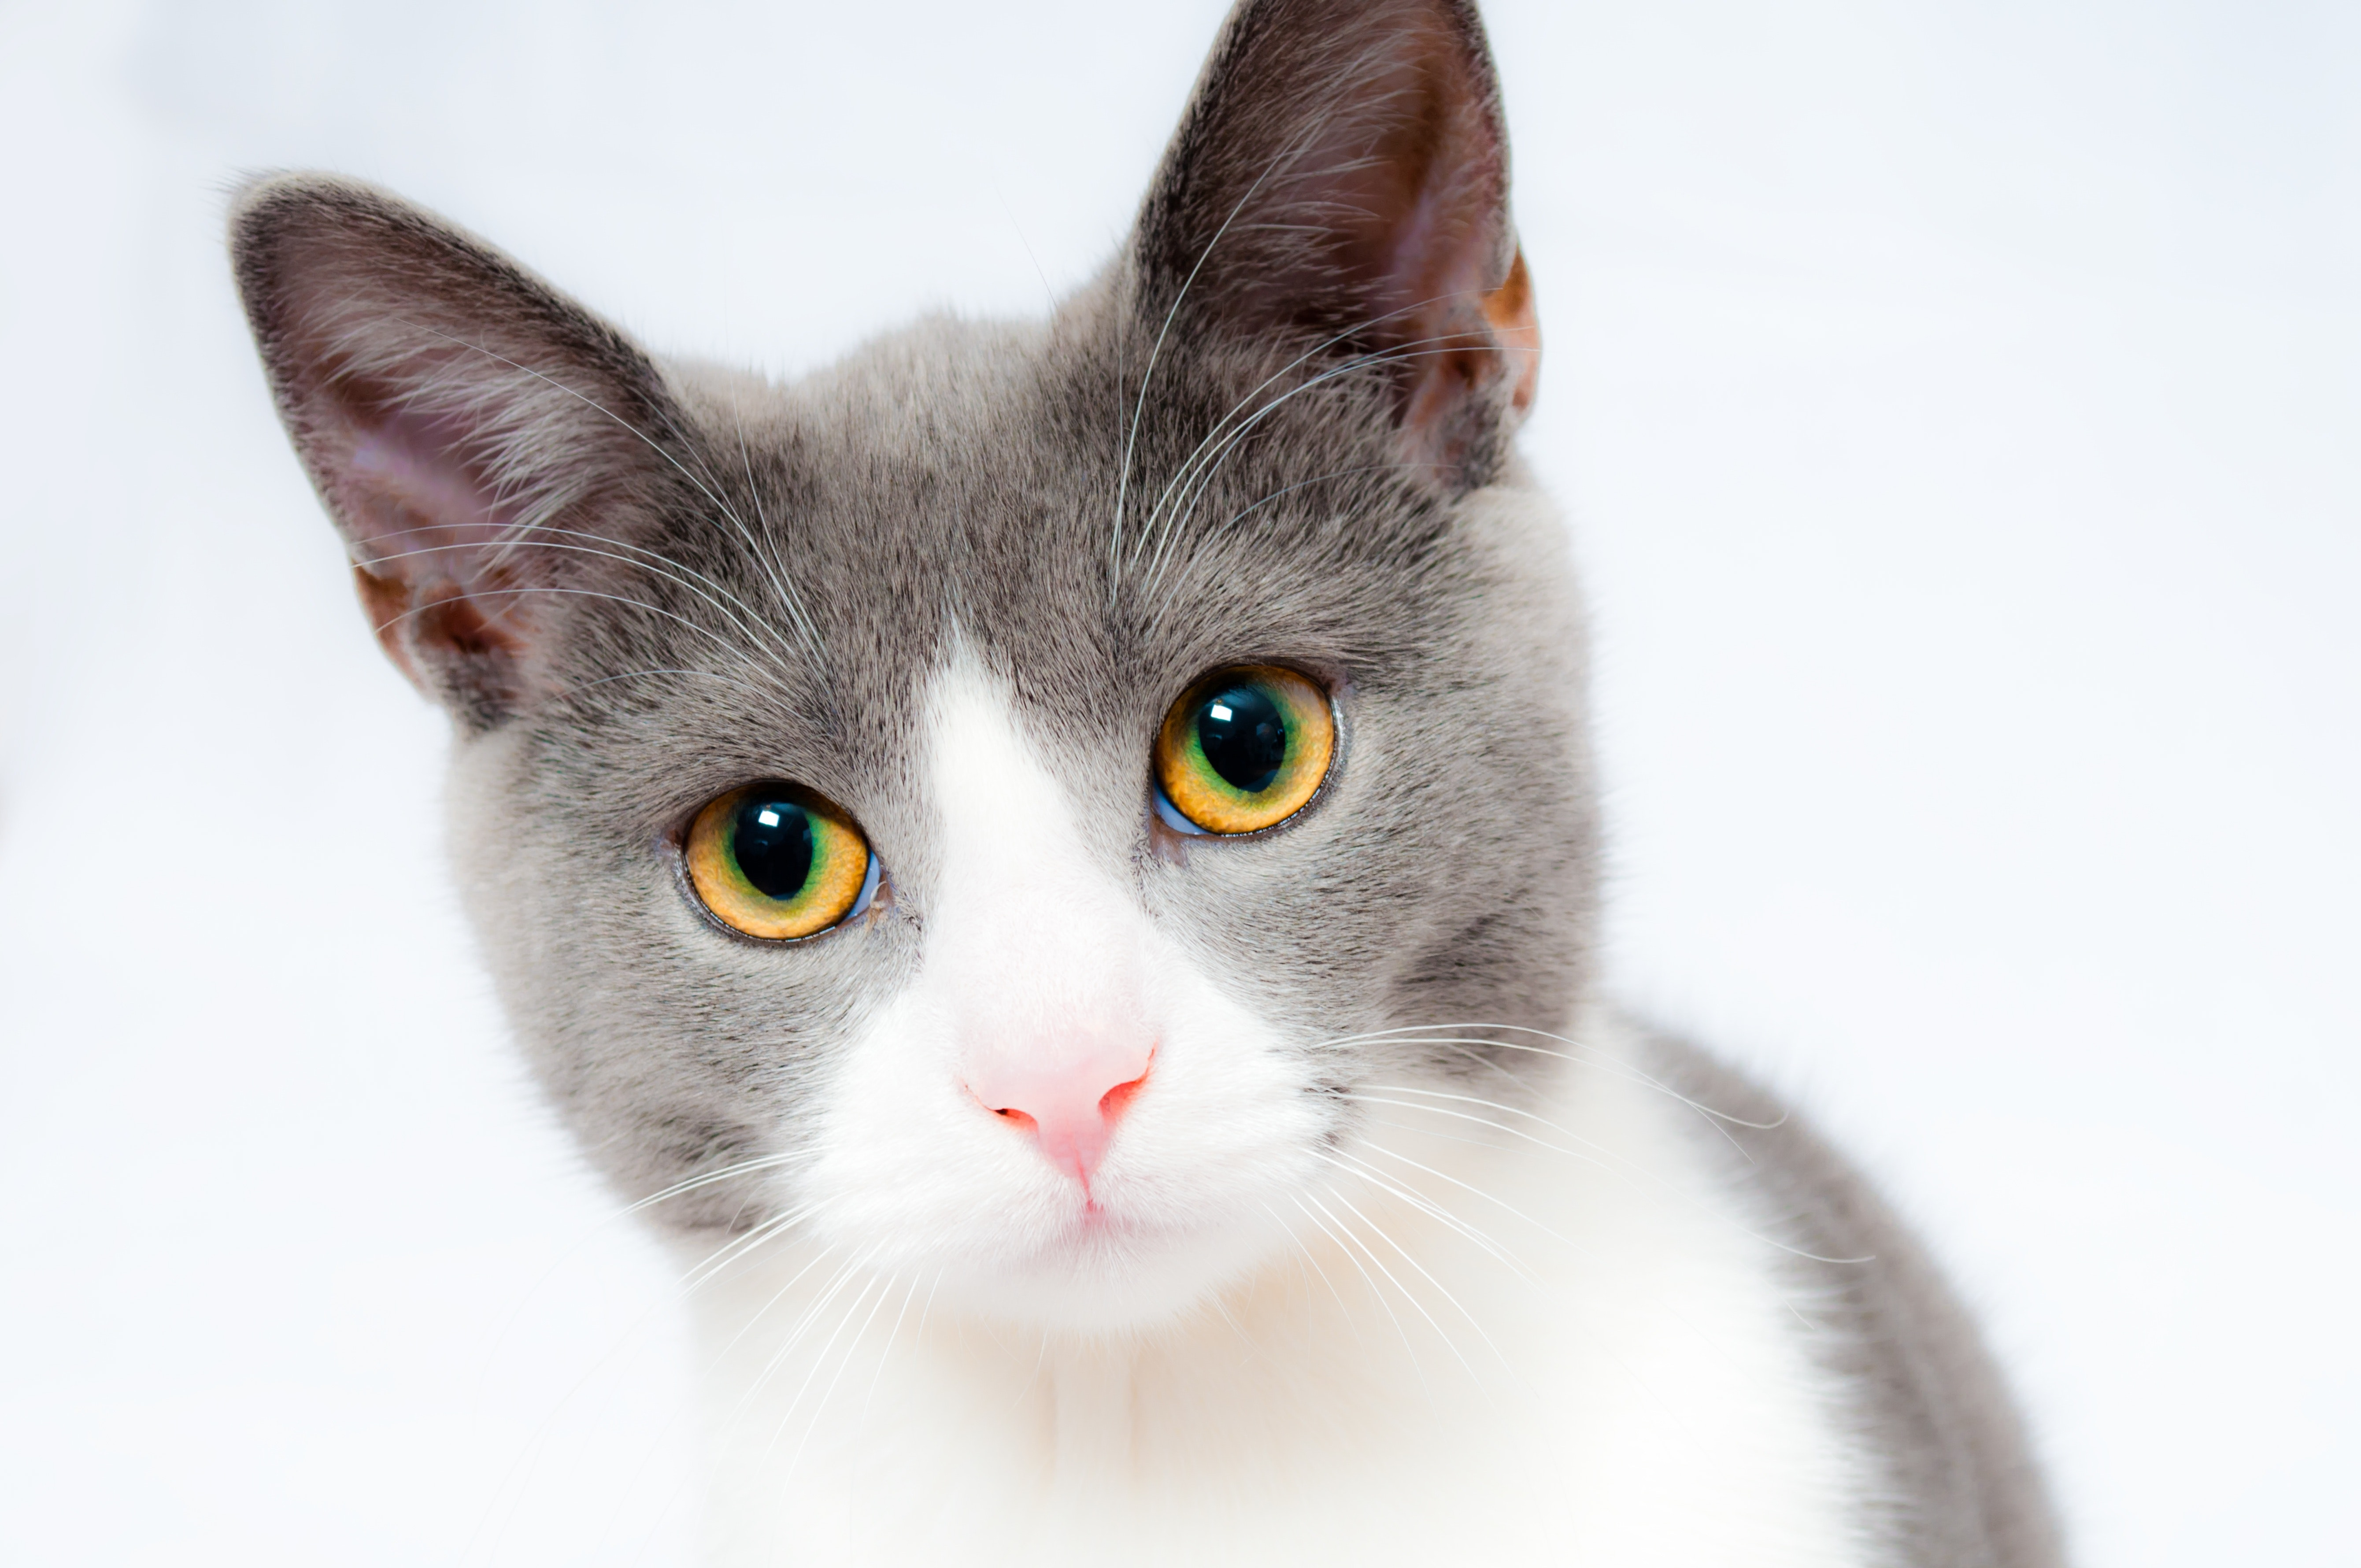
\includegraphics[width=3.5in]{img/test1_cat.jpg}
\caption{This is the image caption}
\label{image_label}
\end{figure}

\bibliographystyle{IEEEtran}
\bibliography{test1.bib}

\end{document}